\zap{
\begin{frame}
% \frametitle{The BIZ Procedure: Heterogeneous and Unknown Sampling Variance}
  Fix $c \le 1-(P^*)^{1/(k-1)}$, $\delta>0$, $P^*>1/k$, $B_1,\ldots,B_k>0$, $n_0$ and let
\begin{equation*}
  \label{eq:qhat}
  \qhat_{tx}(A) = 
  \exp\left(\delta\frac{\sum_{x''\in A} \,n_{tx''}}{\sum_{x''\in A}\sigmahat^2_{tx''}} \,\frac{Y_{n_{tx},x}}{n_{tx}}\right) \bigg/
  \sum_{x' \in A}
  \exp\left(\delta\,\frac{\sum_{x''\in A} n_{tx''}}{\sum_{x''\in A}\sigmahat^2_{tx''}}\, \frac{Y_{n_{tx'},x'}}{n_{tx'}}\right).
\end{equation*}

\bit
\item[1.] Sample each alternative $n_0$ times.  For each $x$, let $n_{0x} \leftarrow n_0$, and let $Y_{0x}$ and $\sigmahat^2_{0x}$ be the sample mean and sample variance respectively.
Also let $A \leftarrow \{ 1,\ldots, k\}$, $\upthresh \leftarrow P^*$, $t \leftarrow 1$.
\item[2.] While $\max_{x\in A} \qhat_{tx}(A) < P$
  \bit
\item[2a.] While $\min_{x\in A} \qhat_{tx}(A) \le c$
  \bit
	\item Let $x \in \argmin_{x\in A} \qhat_{tx}(A)$.
	\item Let $\upthresh \leftarrow \upthresh/(1-\qhat_{tx}(A))$.
	\item Remove $x$ from $A$.
   \eit
 \item[2b.] Let $z \in \argmin_{x\in A} n_{tx} / \sigmahat^2_{tx}$.
 \item[2c.] For each $x\in A$, let 
    $n_{t+1,x} = \ceil\left( \sigmahat^2_{tx} (n_{tz} + B_z) / \sigmahat^2_{tz} \right)$.
  \item[2d.] For each $x\in A$, if $n_{t+1,x}>n_{tx}$, take $n_{t+1,x}-n_{tx}$ additional samples from alternative $x$.  Let $Y_{t+1,x}$ and $\sigmahat^2_{t+1,x}$ be the sample mean and sample variance respectively of all samples from alternative $x$ thus far.  Then increment $t$.
\eit
\item[3.] Select $\xhat \in \argmax_{x\in A} Y_{tx} / n_{tx}$ as our estimate of the best.
\eit
\end{frame}


\begin{frame}
  \frametitle{Continuation Region}
  \begin{itemize}
    \item Images show continuation region for $k=3$, \\ in linear coordinates (left) and exponential coordinates (right).  
    \item BKS (BIZ with $c=0$) stops when $Y_t$ exits the continuation region.
  \end{itemize}
  \begin{figure}
  \center{
  \includegraphics[width=2in]{\figdir/BayesIZ/ContinuationRegion.pdf}
  \quad
  \includegraphics[width=2in]{\figdir/BayesIZ/ContinuationRegionGBM.pdf}
  }
  \end{figure}
\end{frame}

\begin{frame}
  \frametitle{Proof Sketch}
  Let $\CS$ be the event of correct selection. \\
  For $\theta\in\R^d$, let $Q_\theta$ be a prior that is uniform on the permutations $\theta$.
  In particular, $Q = Q_{[\delta,0,\ldots,0]}$.

  \begin{lemma}[Symmetry]
    %$\PCS(\pi,\theta) = Q_\theta\left\{ \text{correct selection under $\pi$} \right\}$ \\
    $\PCS(\pi,\theta)$ is invariant to permutations of $\theta$.  \\ Moreover, $\PCS(\pi,\theta) = Q^\pi_\theta\left\{ \CS \right\}$.
  \end{lemma}
  % \begin{proof}
    % Proof uses a symmetry or ``equalizing'' argument.
  % \end{proof}

  % The first, Lemma~\ref{l:correspondence}, shows that the non-Bayesian
  % probability of correct selection $\PCS(\pi,u)$ is identical to the probability
  % of correct selection under the Bayesian prior $Q_u$.  The proof follows a
  % symmetry or ``equalizing'' argument.

  \begin{lemma}[Monotonicity]
    For $\theta\in\PZ(\delta)$, 
    $Q^\pi_\theta\{CS\} \ge Q^\pi_{[\delta,0,\ldots,0]}\{CS\}$.
  \end{lemma}
   % monotonicity argument dealing directly with the form of the posterior probabilities.

   \begin{lemma}[Bayes PCS of Least-favorable Configuration]
    $Q^\pi_{[\delta,0,\ldots,0]}\{CS\} \ge P^*$, with equality if $\T=\R_+$.
   \end{lemma}
\end{frame}



\begin{frame}
  \frametitle{Generalization of BIZ, which allows sampling in discrete or continuous time} 
  \begin{itemize}
    \item {\bf Parameters}: $\T \in \{\R_+,\Z_+\}$, $c \le 1 - (P^*)^{1/(k-1)}$, $\delta>0$, $P^*>1/k$.
    \item {\bf Initalization}: $\tau_0 = 0$, $A_0=\{1,\ldots,k\}$, $\upthresh_0 = P^*$.
\item {\bf Elimination Time}: 
  \begin{multline*}
  \tau_{n+1} = \inf\left\{ t \in \T \cap [\tau_n,\infty) : 
  \min_{x\in A_n} q_{tx}(A_n) \le c 
  %\right. \\ \left. 
  \text{ or } 
  \max_{x\in A_n} q_{tx}(A_n) \ge \upthresh_n \right\}.
  \end{multline*}
\item {\bf Eliminated Alternative and Contention Set}:
  \begin{equation*}
    Z_{n+1} = \argmin_{x\in A_n} q_{\tau_{n+1}}(A_n), \qquad
    A_{n+1} = A_n \setminus Z_{n+1}
  \end{equation*}
\item {\bf Stopping Boundary}: 
  \begin{equation*}
    \upthresh_{n+1} = \upthresh_n \bigg/ \left(1 - \min_{x\in A_n} q_{\tau_{n+1}}(A_n)\right).
  \end{equation*}
\item The {\bf selected alternative} is the single alternative in $A_{k-1}$.
\end{itemize}
\end{frame}


\zap{
\begin{frame}
  \frametitle{We construct BIZ with Bayesian ideas \ldots \\ 
  \ldots but BIZ is a non-Bayesian Method}
    \begin{itemize}
      \item BIZ is motived using Bayesian ideas, and manipulation of Bayesian PCS is critical in proofs of theoretical results.
      \item However, BIZ is a non-Bayesian method.
      \item You do not need to have a prior to use BIZ, and its IZ guarantee is non-Bayesian.
  \end{itemize}
\end{frame}
}


\begin{frame}
\frametitle{Heterogeneous Sampling Variance: Continuous Time}
\begin{itemize}
  \item In general, sampling variances $\sigma_x^2$ are heterogeneous and unknown.
  \item In continuous time, this problem is easily addressed:
    \begin{enumerate}
  \item The sampling variance $\sigma^2_x$ can be estimated perfectly given $(Y_{tx} : 0\le t \le \epsilon)$ for any $\epsilon > 0$. 
  \item Replace $Y_{t,x} \sim \Ncal(\theta_x,t\sigma^2_x)$ with $Y_{\sigma_x^2 t,x} / \sigma_x^2 \sim \Ncal(\theta_x,t)$ and we obtain a ranking and selection problem with common sampling variance $1$.
  \item Use BIZ for common sampling variance $1$ on the transformed $Y$ values.
\end{enumerate}
  \item The IZ guarantee and the tightness of the PCS bound still hold.
\end{itemize}
\end{frame}

\begin{frame}
\frametitle{Heterogeneous and Unknown Sampling Variance: \\ Discrete Time}
\begin{itemize}
  \item In discrete time, the problem is harder:
  \item Idea: use a discrete-time approximation to $Y_{\sigma_x^2 t,x} / \sigma_x^2$ in our calculation of $q_{tx}(A)$, based on the sample variances $\sigmahat^2_x$.
  \item When this discrete-time approximation is exact, we retain the IZ guarantee.
  \item When it does not hold, the IZ guarantee no longer holds, and the procedure is a heuristic.
  \item Ongoing work: Does the IZ guarantee hold in a limiting sense?
  %\item Let $n_{tx}$ be the number of samples taken from alternative $x$ by time $t$. 
  %\item Keep $n_{tx}$ proportional to $\sigmahat^2_x$ (as much as allowed by discrete time).
  %\item Most obvious approach:  Then, use $Y_{n_{tx},x} / \sigmahat^2_x$ as our approximation to 
%$Y_{\sigma_x^2 t,x} / \sigma_x^2$
  %\item A better approach: use
    %\begin{equation*}
    %\frac{\sum_{x'\in A} \,n_{tx'}}{\sum_{x'\in A}\sigmahat^2_{tx'}} \,\frac{Y_{n_{tx},x}}{n_{tx}}
    %\end{equation*}
  %\item When $n_{tx}$ is exactly proportional to $\sigma^2_x$ and $\sigmahat^2_x = \sigma^2_x$, this reduces to what we had in continuous time, and the IZ guarantee still holds.
  %\item Otherwise, the IZ guarantee does not hold, and the procedure is a heuristic.
  %\item Ongoing work: Does the IZ guarantee hold in a limiting sense?
\end{itemize}
\end{frame}


\begin{frame}
\frametitle{Heterogeneous and Unknown Sampling Variance: \\ Discrete Time}
\begin{itemize}
  \item Let $n_{tx}$ be the number of samples taken from alternative $x$ by time $t$. 
  \item We sample so as to keep $n_{tx}$ proportional to $\sigmahat^2_x$ (as much as allowed by discrete time).
  \item Most obvious approach:  Approximate $Y_{\sigma_x^2 t,x} / \sigma_x^2$
    with $Y_{n_{tx},x} / \sigmahat^2_x$.
  \item A better approach: approximate it with
    \begin{equation*}
      \frac{\sum_{x'\in A} \,n_{tx'}}{\sum_{x'\in A}\sigmahat^2_{tx'}} \,\frac{Y_{n_{tx},x}}{n_{tx}}
    \end{equation*}
  This allows the alternative with the highest $q_{tx}(A)$ to also be the one with the highest sample mean, $Y_{n_{tx},x}/n_{tx}$.
  \item When $n_{tx}$ is exactly proportional to $\sigma^2_x$ and $\sigmahat^2_x = \sigma^2_x$, this reduces to what we had in continuous time, and the IZ guarantee still holds.
  % \item Otherwise, the IZ guarantee does not hold, and the procedure is a heuristic.
  % \item Ongoing work: Does the IZ guarantee hold in a limiting sense?
\end{itemize}
\end{frame}



  % \REQUIRE $c \in [0,\cmax]$, $\delta>0$, $P^*\in(1/k,1)$, $n_0\ge0$ an integer, $B_1,\ldots,B_k$ strictly positive integers.  Recommended choices are $c=\cmax$, $B_1=\cdots=B_k=1$ and $n_0 = 100$.
    % $\sigmahat^2_{tx}$ with the true values $\lambda^2_x$, and set $n_0=0$.
    % To compute $\qhat_{tx}(A)$, use \eqref{eq:qhat}.


\begin{frame}
  \frametitle{Unknown Heterogeneous Variance}
  Slippage configuration.\\
  Top row: increasing variance.  Bottom row: decreasing variance.\\
  Left column: $E[N]/k$.  Right column: PCS.\\
  \begin{figure}
    \center
    % 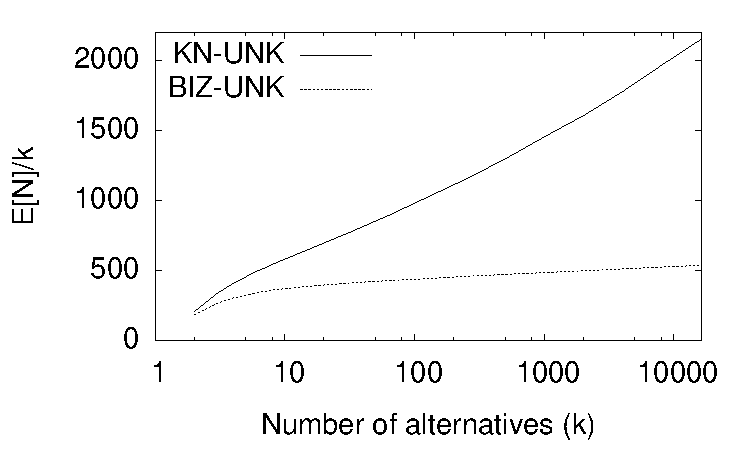
\includegraphics[width=2in]{\figdir/BayesIZ/FINAL-UNK-SC-Nk} 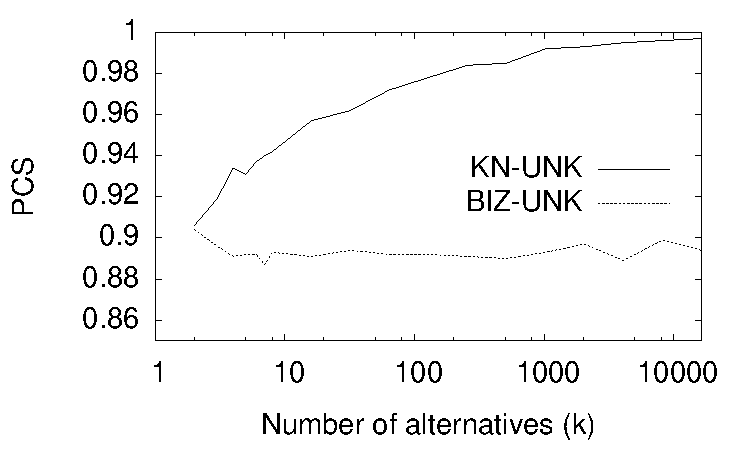
\includegraphics[width=2in]{\figdir/BayesIZ/FINAL-UNK-SC-PCS}\\
    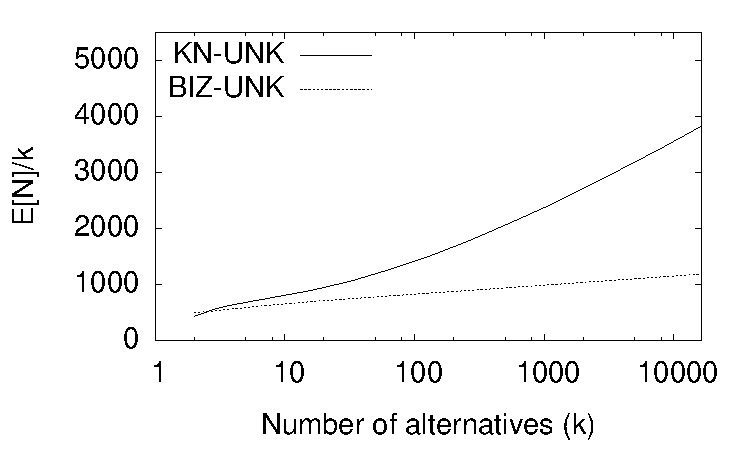
\includegraphics[width=2in]{\figdir/BayesIZ/FINAL-UNK-SCINC-Nk} 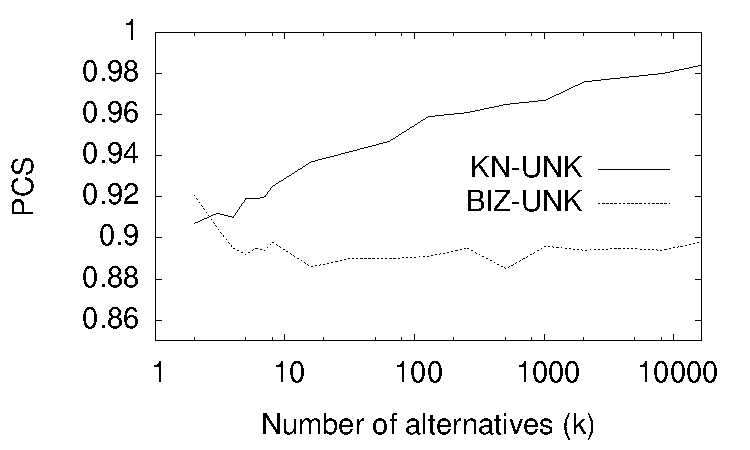
\includegraphics[width=2in]{\figdir/BayesIZ/FINAL-UNK-SCINC-PCS}\\
    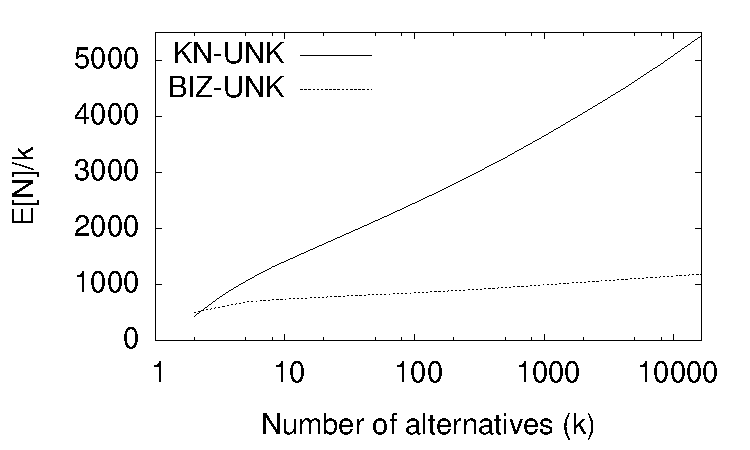
\includegraphics[width=2in]{\figdir/BayesIZ/FINAL-UNK-SCDEC-Nk} 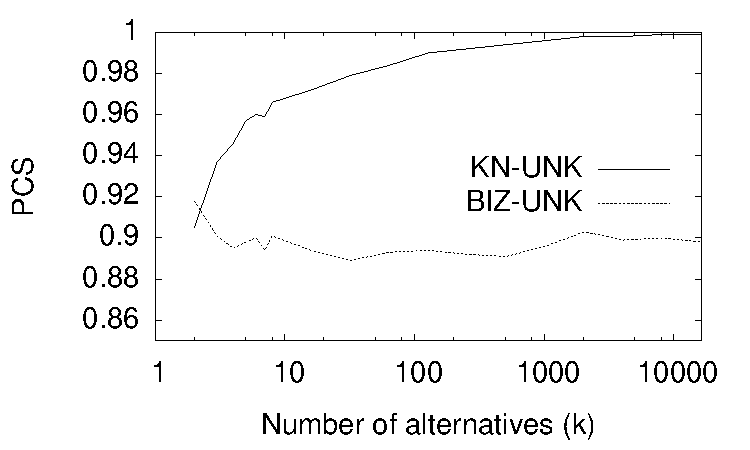
\includegraphics[width=2in]{\figdir/BayesIZ/FINAL-UNK-SCDEC-PCS}\\
    % {\bf MDM-INC} 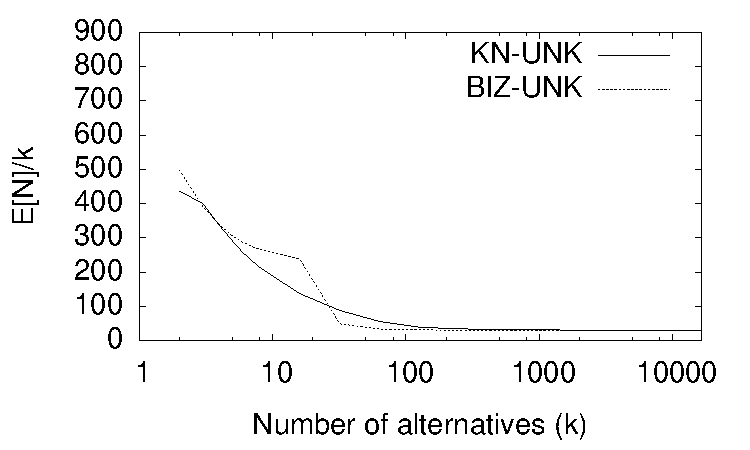
\includegraphics[width=2in]{\figdir/BayesIZ/FINAL-UNK-MDMINC-Nk} 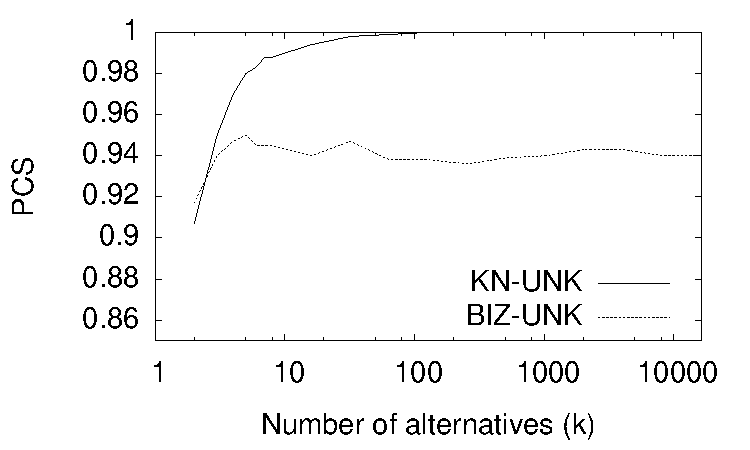
\includegraphics[width=2in]{\figdir/BayesIZ/FINAL-UNK-MDMINC-PCS}\\
    % {\bf MDM-DEC} 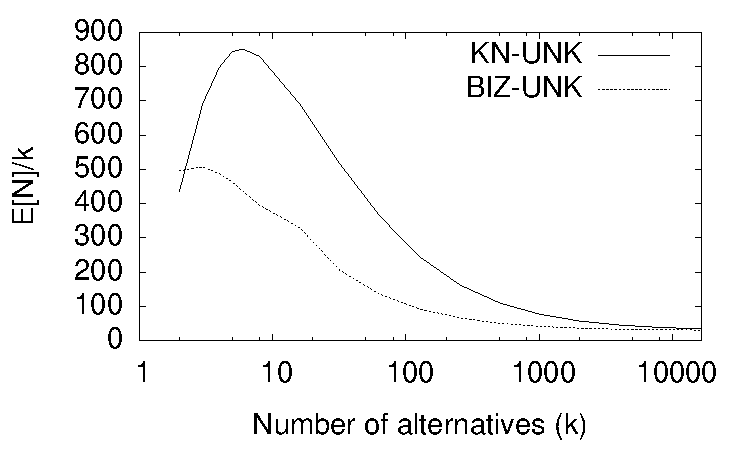
\includegraphics[width=2.7in]{\figdir/BayesIZ/FINAL-UNK-MDMDEC-Nk} 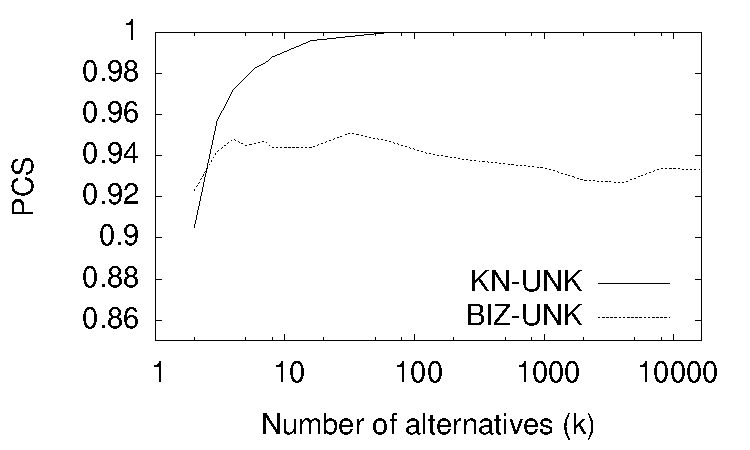
\includegraphics[width=2.7in]{\figdir/BayesIZ/FINAL-UNK-MDMDEC-PCS}\\
    % {\bf RPI-HET} 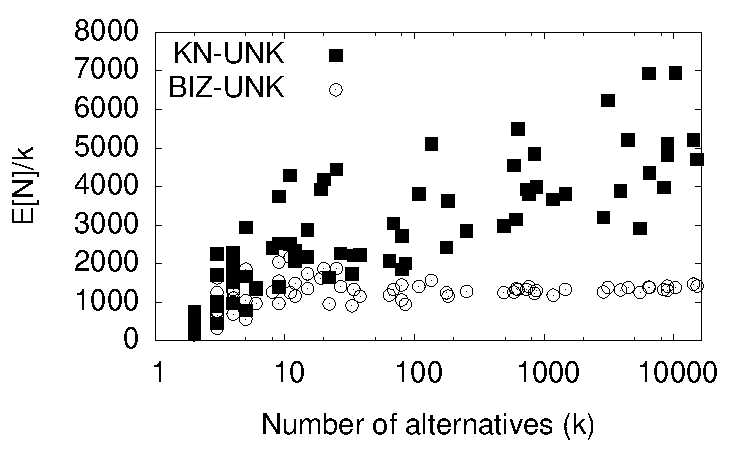
\includegraphics[width=2.7in]{\figdir/BayesIZ/FINAL-UNK-RPIHET-Nk} 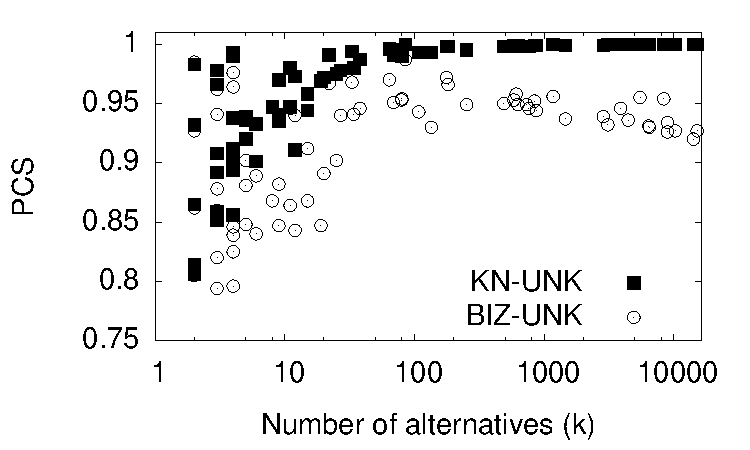
\includegraphics[width=2.7in]{\figdir/BayesIZ/FINAL-UNK-RPIHET-PCS}\\
  \end{figure}

    %Row shows PCS and $E[N]/k$ as a function of the number of alternatives $k$ under the following configurations:
    %SC-INC (row 1); SC-DEC (row 2); MDM-INC (row 3); MDM-DEC (row 4); and RPI-HET (row 5).
    %In all configurations, $P^*=0.8$, $\sigma=10$, $\delta=0.5$, and the sampling variances are unknown.
\end{frame}

\begin{frame}
  \frametitle{Unknown Heterogeneous Variance}
  Monotone Decreasing Means configuration.\\
  Top row: increasing variance.  Bottom row: decreasing variance.\\
  Left column: $E[N]/k$.  Right column: PCS.\\
  \begin{figure}
    \center
    % 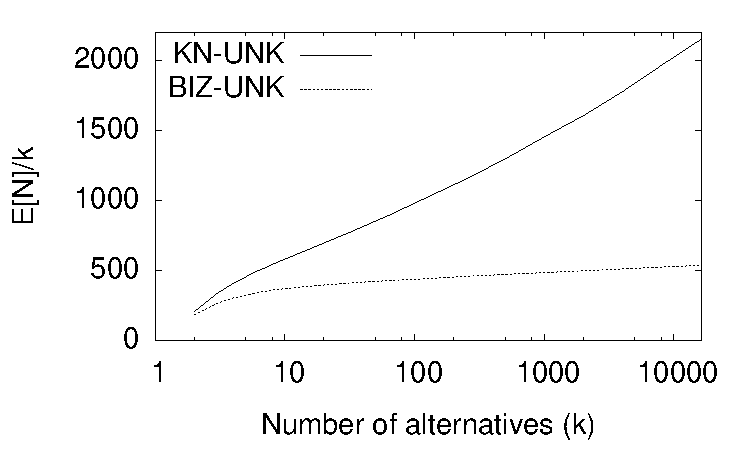
\includegraphics[width=2in]{\figdir/BayesIZ/FINAL-UNK-SC-Nk} 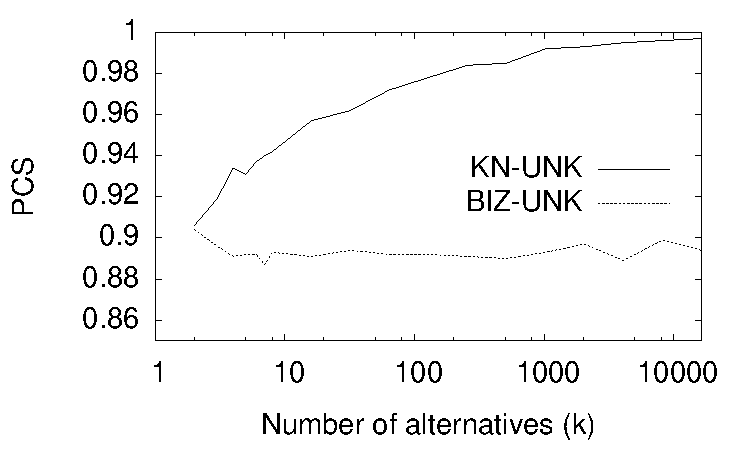
\includegraphics[width=2in]{\figdir/BayesIZ/FINAL-UNK-SC-PCS}\\
    %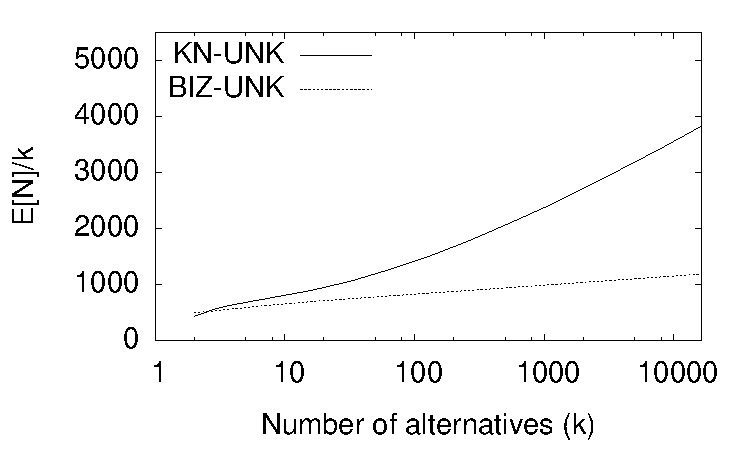
\includegraphics[width=2in]{\figdir/BayesIZ/FINAL-UNK-SCINC-Nk} 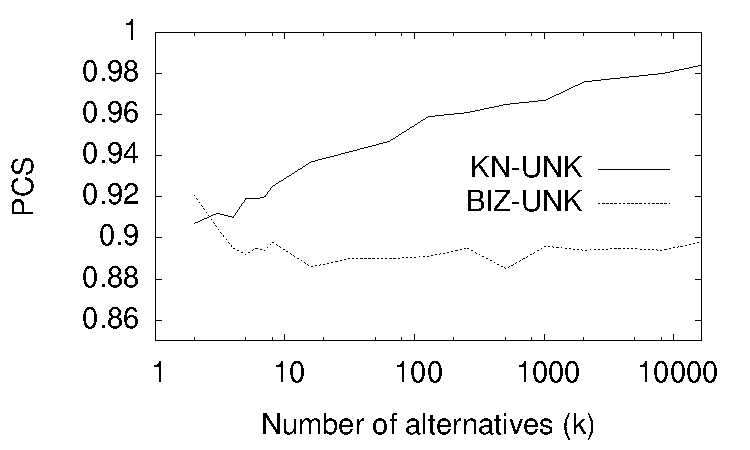
\includegraphics[width=2in]{\figdir/BayesIZ/FINAL-UNK-SCINC-PCS}\\
    %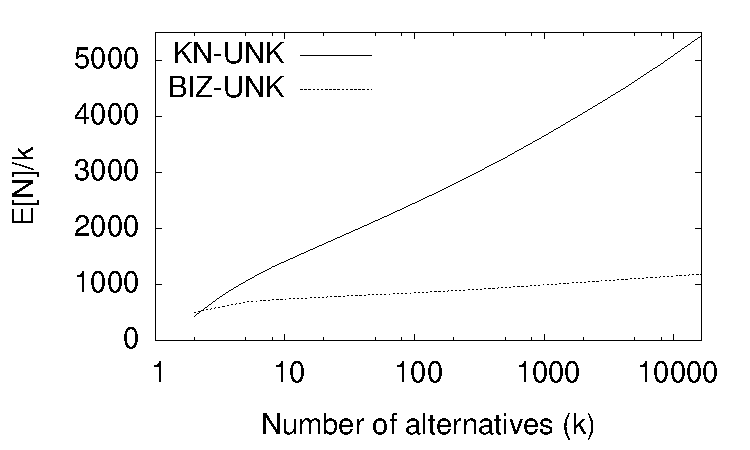
\includegraphics[width=2in]{\figdir/BayesIZ/FINAL-UNK-SCDEC-Nk} 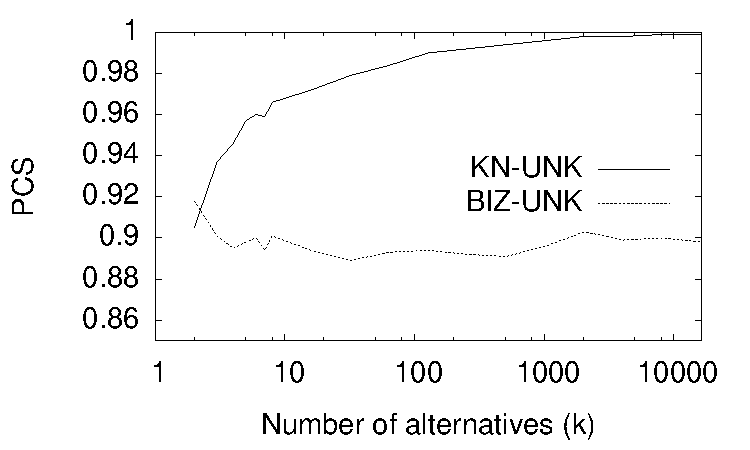
\includegraphics[width=2in]{\figdir/BayesIZ/FINAL-UNK-SCDEC-PCS}\\
    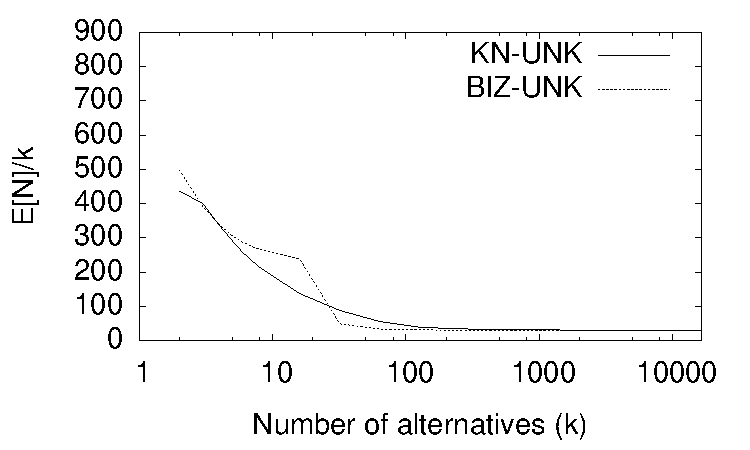
\includegraphics[width=2in]{\figdir/BayesIZ/FINAL-UNK-MDMINC-Nk} 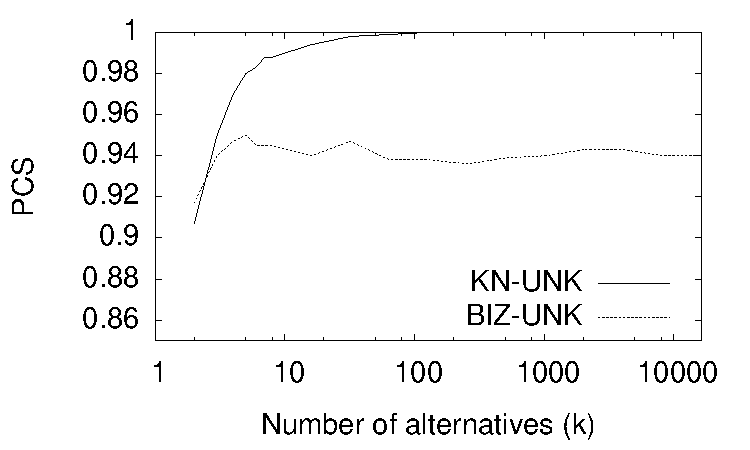
\includegraphics[width=2in]{\figdir/BayesIZ/FINAL-UNK-MDMINC-PCS}\\
    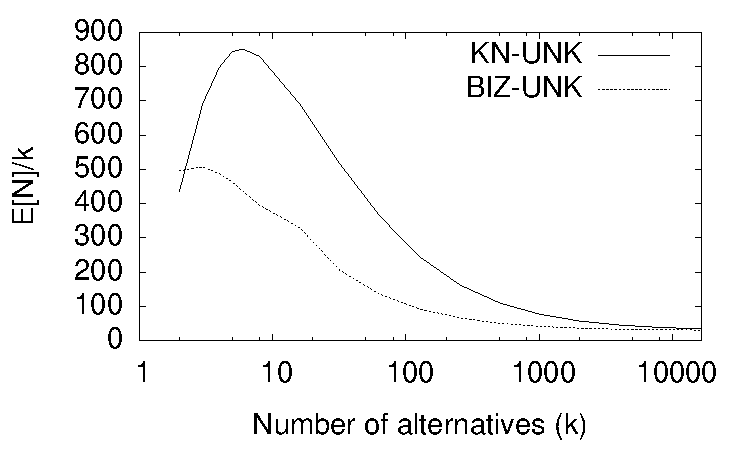
\includegraphics[width=2in]{\figdir/BayesIZ/FINAL-UNK-MDMDEC-Nk} 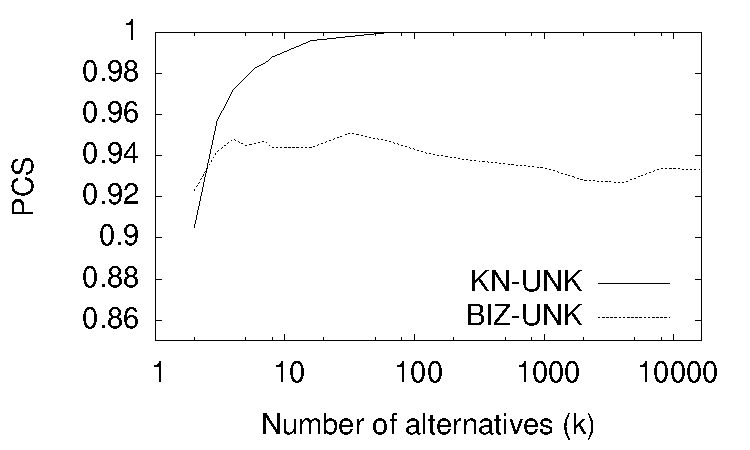
\includegraphics[width=2in]{\figdir/BayesIZ/FINAL-UNK-MDMDEC-PCS}\\
    % {\bf RPI-HET} 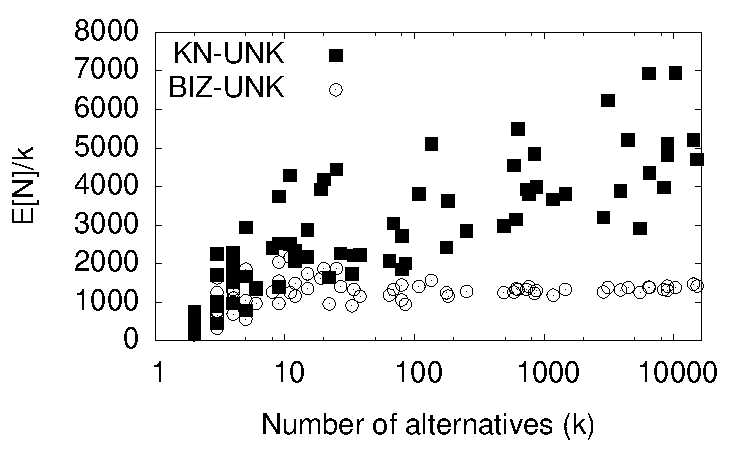
\includegraphics[width=2.7in]{\figdir/BayesIZ/FINAL-UNK-RPIHET-Nk} 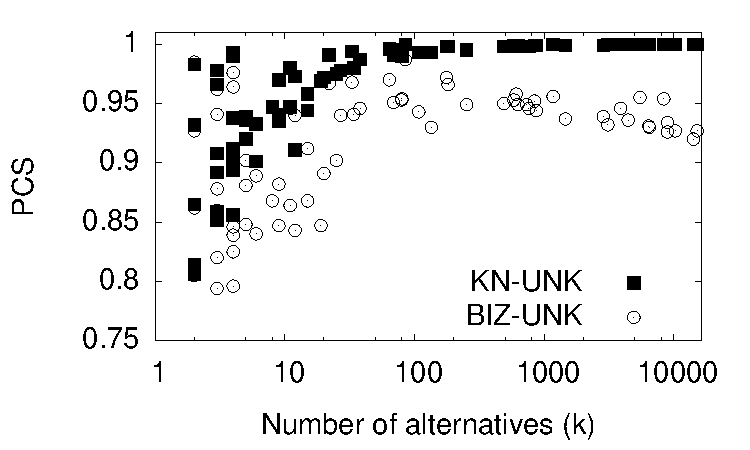
\includegraphics[width=2.7in]{\figdir/BayesIZ/FINAL-UNK-RPIHET-PCS}\\
  \end{figure}
\end{frame}

\begin{frame}
  \frametitle{Unknown Heterogeneous Variance}
  Random Problem Instances.  \\
  Top row: common variance.  Bottom row: heterogeneous variance.\\
  Left column: $E[N]/k$.  Right column: PCS.\\
  \begin{figure}
    \center
    % 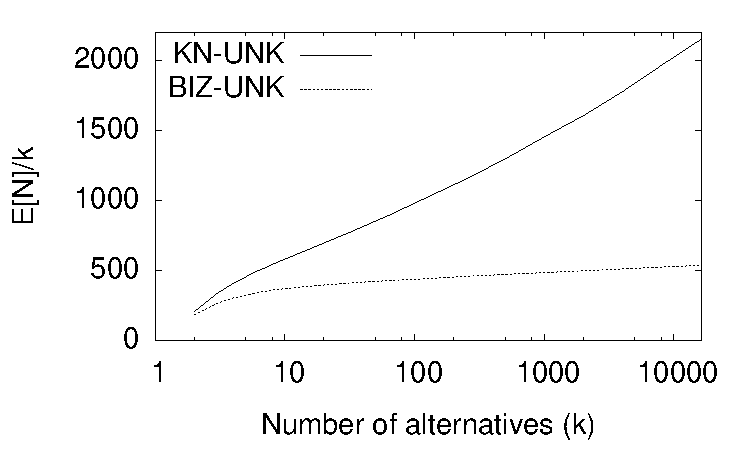
\includegraphics[width=2in]{\figdir/BayesIZ/FINAL-UNK-SC-Nk} 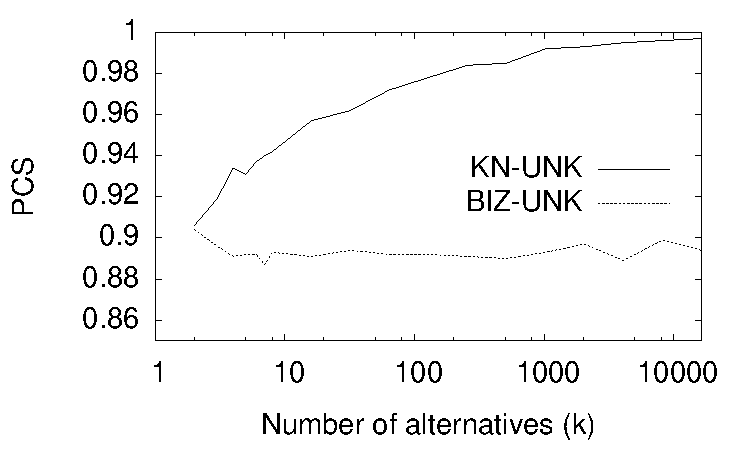
\includegraphics[width=2in]{\figdir/BayesIZ/FINAL-UNK-SC-PCS}\\
    %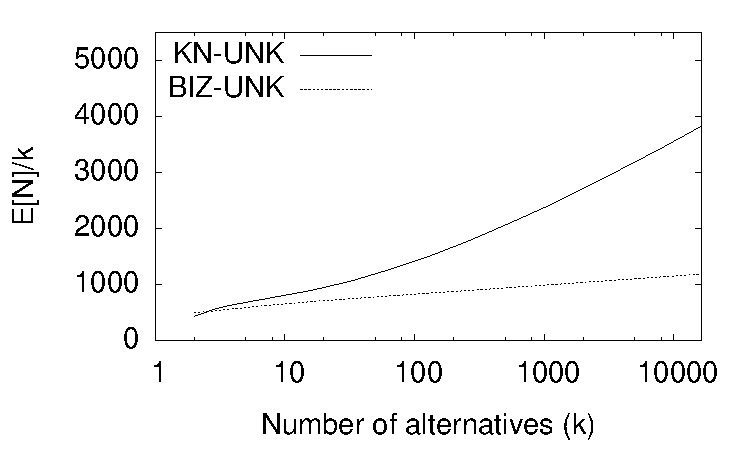
\includegraphics[width=2in]{\figdir/BayesIZ/FINAL-UNK-SCINC-Nk} 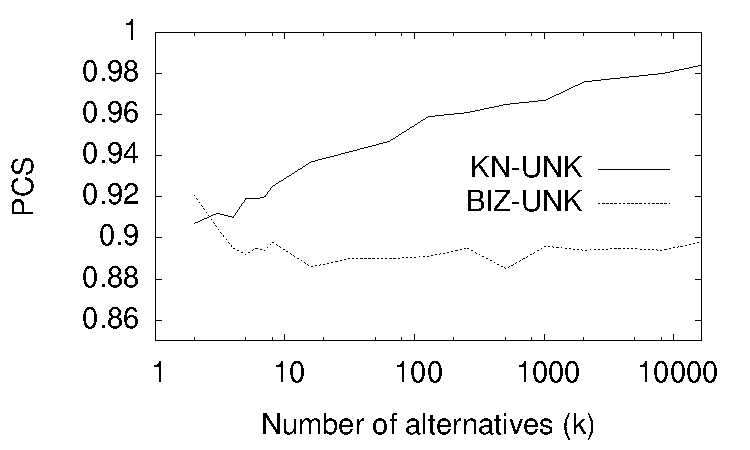
\includegraphics[width=2in]{\figdir/BayesIZ/FINAL-UNK-SCINC-PCS}\\
    %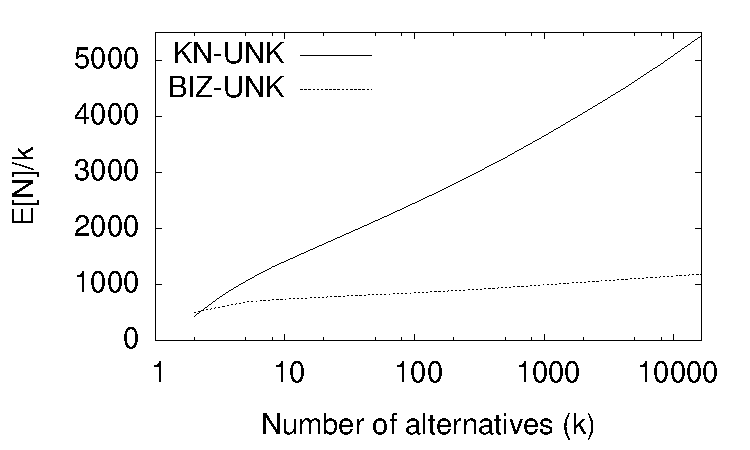
\includegraphics[width=2in]{\figdir/BayesIZ/FINAL-UNK-SCDEC-Nk} 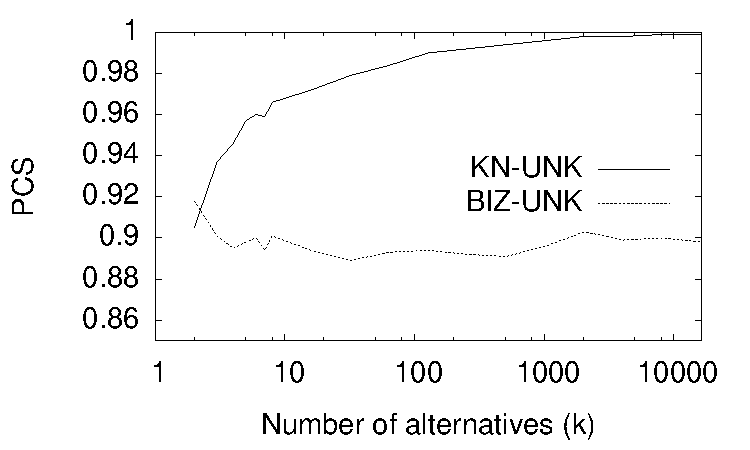
\includegraphics[width=2in]{\figdir/BayesIZ/FINAL-UNK-SCDEC-PCS}\\
    %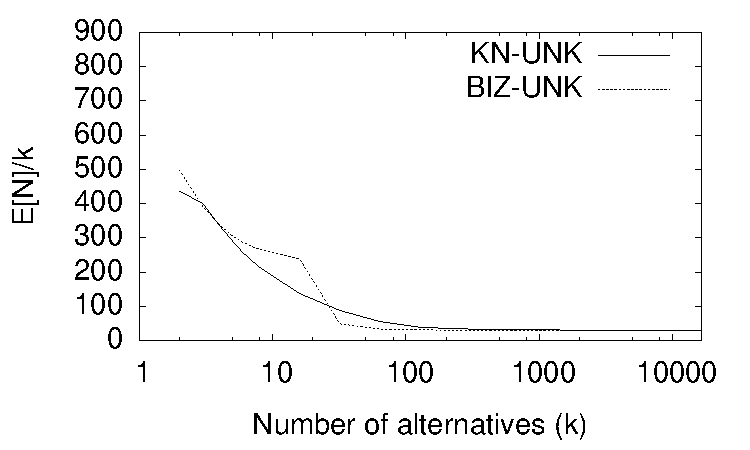
\includegraphics[width=2in]{\figdir/BayesIZ/FINAL-UNK-MDMINC-Nk} 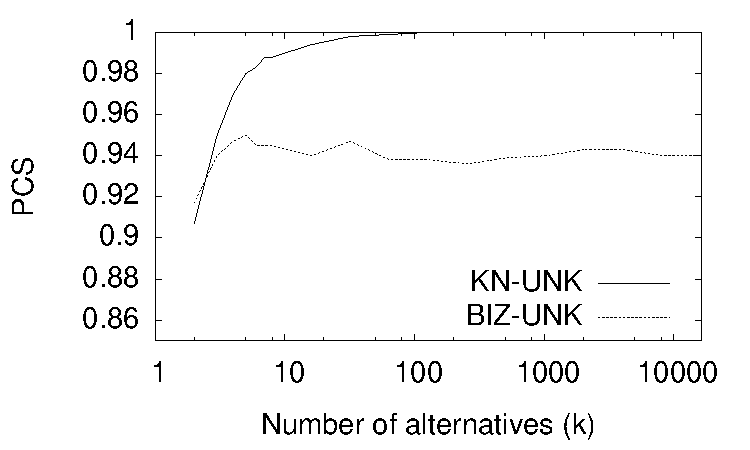
\includegraphics[width=2in]{\figdir/BayesIZ/FINAL-UNK-MDMINC-PCS}\\
    %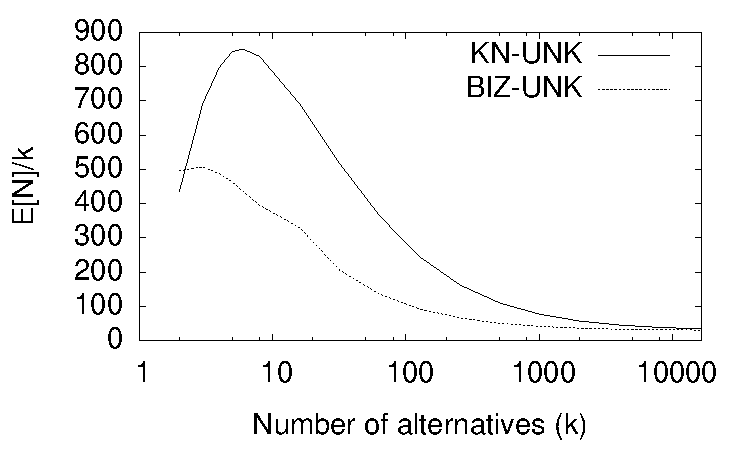
\includegraphics[width=2in]{\figdir/BayesIZ/FINAL-UNK-MDMDEC-Nk} 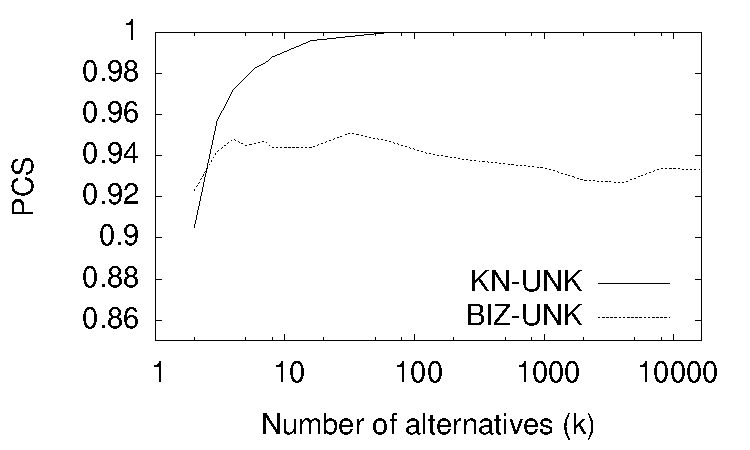
\includegraphics[width=2in]{\figdir/BayesIZ/FINAL-UNK-MDMDEC-PCS}\\
    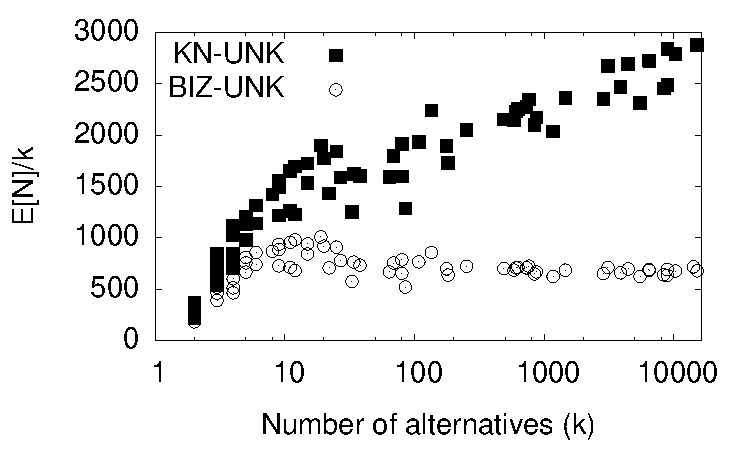
\includegraphics[width=2in]{\figdir/BayesIZ/FINAL-UNK-RPI-Nk} 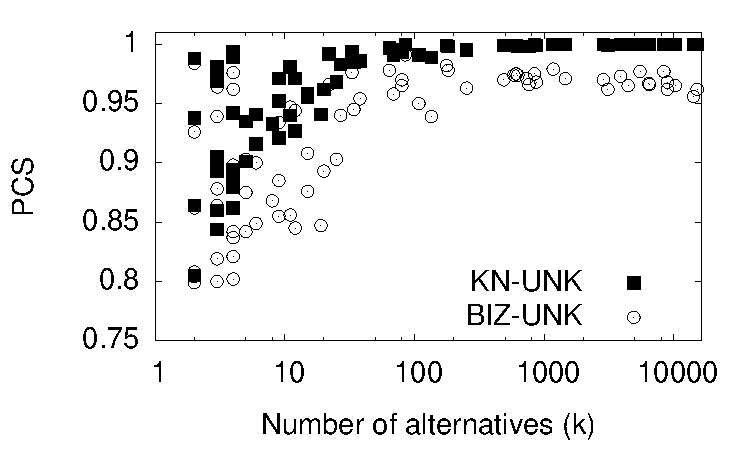
\includegraphics[width=2in]{\figdir/BayesIZ/FINAL-UNK-RPI-PCS}\\
    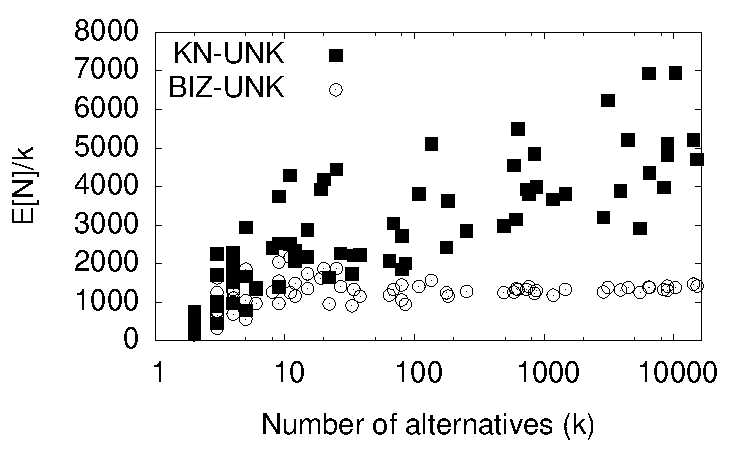
\includegraphics[width=2in]{\figdir/BayesIZ/FINAL-UNK-RPIHET-Nk} 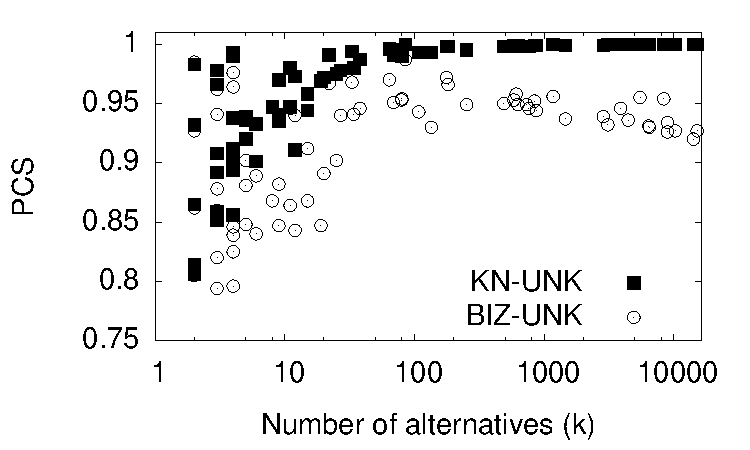
\includegraphics[width=2in]{\figdir/BayesIZ/FINAL-UNK-RPIHET-PCS}\\
  \end{figure}
\end{frame}

\begin{frame}
  \frametitle{Tight PCS Bounds}
  \begin{theorem}
  Assume that $\sigma^2_x = \sigma^2$ is known.
  Fix any $\delta>0$, $P^* \in (1/k,1)$, $c \le 1-(P^*)^{1/(k-1)}$, $\T \in \{\R_+,\Z_+\}$, 
  and let sampling occur under BIZ.
  Then,
    \begin{equation*}
      \PCS(\theta) \ge P^*\quad \forall \theta\in\PZ(\delta)
    \end{equation*}
    Moreover, for a continuous-time generalization of BIZ,
    \begin{equation*}
      \inf_{\theta\in\PZ(\delta)} \PCS(\theta) = P^*
    \end{equation*}
  \end{theorem}
\end{frame}

\begin{frame}
  \begin{figure}
    \centering
    \includegraphics[width=4.2in]{\figdir/BayesIZ/ALL_01_2013a.pdf} 
  \end{figure}
\end{frame}


}


\zap{
\begin{frame}\frametitle{Loose PCS bounds cause the
the number of samples taken to be larger than necessary}
\begin{columns}[l]
\column{1.5in}
	\begin{figure}
	\center
	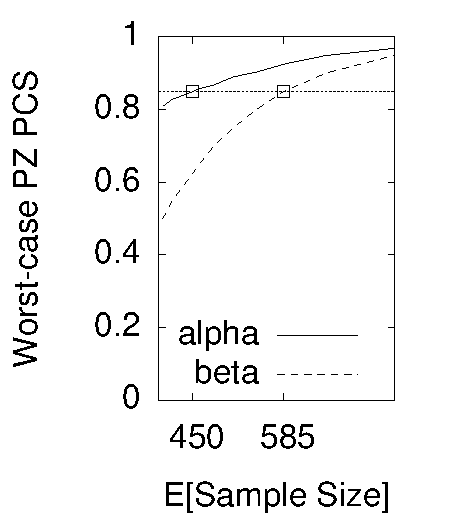
\includegraphics[width=2in]{\figdir/BayesIZ/ICS2013_overdelivery2.pdf}
	\end{figure}
\column{3in}
\begin{itemize}
  \item Consider a sampling procedure with a tunable parameter $h$, that controls how much sampling is done.
  \item If we increase $h$, then $\pi(h)$ takes more samples, and provides a bigger PCS.
  \item Let $\alpha(h) = \inf_{\theta \in \PZ(\delta)} \PCS(\pi(h),\theta)$ be the actual worst-case preference-zone PCS.  (solid line, from exhaustive simulation)
  \item Let $\beta(h) \le \alpha(h)$ be the best bound on $\alpha(h)$ that we can prove.  (dashed line)
  \item We choose $h$ so that $\beta(h) = P^*$.
  \item Had we known $\alpha$, we could have instead chosen a smaller $h$ with $\alpha(h) = P^*$, and taken fewer samples. 
  % \item Loose bounds cause the number of samples taken to be larger than necessary.
\end{itemize}
\end{columns}
\end{frame}
}

\zap{
\begin{frame}
\frametitle{Loose PCS Bounds Lead To Oversampling}
\center
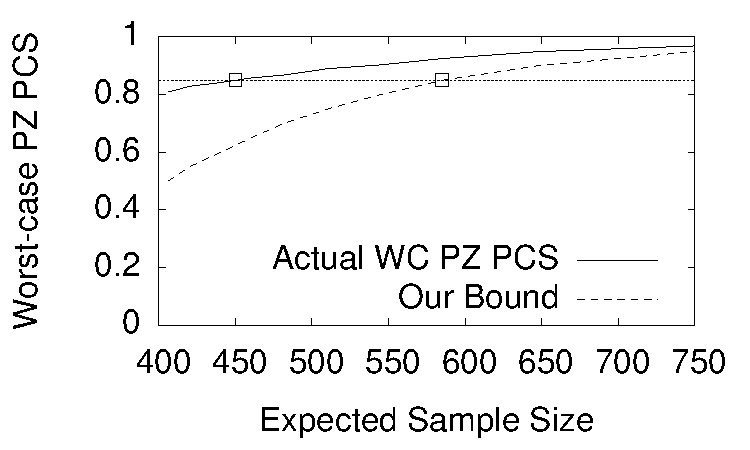
\includegraphics[width=3.5in]{\figdir/BayesIZ/ICS2013_overdelivery.pdf} \\
\bit
\item The procedure we would use is the one where the horizontal line at $0.85$ crosses the dashed line, expected sample size 575.
\item Had our bounds been perfect, we would have used the one where the horizontal line crosses the solid line, expected sample size 450.
% \item (results from KN, $k=32$ alternatives)
\eit
\end{frame}
}


\zap{
\begin{frame}
  \frametitle{Loose PCS Bounds Lead To Oversampling}
% A common criticism of policies with IZ guarantees is that they are
% ``difficult to control'' and take too many samples for the desired level of PCS.
\begin{itemize}
  \item Let $\pi$ be a procedure with an IZ guarantee for a fixed $P^*$ and $\delta$.
  \item $P^*$ is the PCS that $\pi$ guarantees it will deliver.
  \item For any $\theta\in\PZ(\delta)$, 
	\begin{equation*}
	\PCS(\pi,\theta) - P^* 
	\end{equation*}
	is the {\bf overdelivery} on PCS.
      % \item For existing policies, there are configurations $\theta$ for which this overdelivery is {\bf significantly} greater than $0$. % large.
      \item Overdelivery on PCS is inefficient: we could have taken fewer samples and achieved the guaranteed PCS faster.
      \item For existing policies and large $k$, this overdelivery causes the number of
	samples to be {\bf significantly} larger than needed.
	% while having a larger PCS is nice, it comes at a cost of having taken more samples.
	% \item Goal: keep $\PCS(\pi,\theta)-P^*$ non-negative and close to $0$.
      \end{itemize}
\end{frame}
}


\zap{
\begin{frame}
  \frametitle{Example}
  \begin{itemize}
  \item In most fully sequential techniques, bounds become very loose as $k$ grows large.
  \begin{itemize}
    \item Example:
      KN (citation)
      $k=10$
      $\delta = 1$
      $\theta = [1,0,\ldots,0]$,
      $P^* = 0.90$.
    \item $\PCS(KN,\theta) \approx 0.98$, Expected number of samples taken is $\approx 5000$
    \item It seems that we could take fewer samples while still meeting $PCS(\pi,\theta)\ge 0.90$.
  \end{itemize}
\item This seems to be due to incidental overdelivery caused by inequalities, e.g., Bonferonni's inequality, used when
  proving the IZ guarantee for particular policies.
  \end{itemize}
\end{frame}
}

\zap{
\begin{frame}
  \frametitle{Example: Too Many Samples}
  % In most (all?) existing R\&S techniques, bounds become very loose as $k$ grows large.
  \center{
  \includegraphics[width=2in]{\figdir/BayesIZ/APS-MDMplotN-KN.pdf} \quad
  \includegraphics[width=2in]{\figdir/BayesIZ/APS-MDMplotPCS-KN.pdf}
  }
  \begin{itemize}
    \item This is the {\bf monotone-decreasing-means configuration}, $\theta=[-\delta,-2\delta,\ldots,-k\delta]$.
    \item Parameters are: $\delta=1$, $\sigma_x=10$, $P^*=0.9$.
    \item The procedure is the KN procedure of \cite{KiNe01}, which is state-of-the-art for problems with not much
      variation in $\sigma^2_x$.  It has been modified to use a known sampling variance.
  \end{itemize}
\end{frame}
}




\zap{
\begin{frame}
  \frametitle{Example}
  \begin{itemize}
  \item In most fully sequential techniques, bounds become very loose as $k$ grows large.
  \begin{itemize}
    \item Example:
      KN (citation)
      $k=10$
      $\delta = 1$
      $\theta = [1,0,\ldots,0]$,
      $P^* = 0.90$.
    \item $\PCS(KN,\theta) \approx 0.98$, Expected number of samples taken is $\approx 5000$
    \item It seems that we could take fewer samples while still meeting $PCS(\pi,\theta)\ge 0.90$.
  \end{itemize}
\item This seems to be due to incidental overdelivery caused by inequalities, e.g., Bonferonni's inequality, used when
  proving the IZ guarantee for particular policies.
  \end{itemize}
\end{frame}
}




\begin{frame}
  \frametitle{Bayesian global optimization}
  \begin{itemize}
    \item We wish to solve an optimization problem
      \begin{equation*}
	\max_{x\in[0,1]^d} f(x).
      \end{equation*}
    \item We begin with a Bayesian prior distribution on $f$.
    \item We have the ability to adaptively choose a sequence of points $x_1,x_2,\ldots$ adaptively, observing
      \begin{equation*}
	y_n = f(x_n) + \epsilon_n,
      \end{equation*}
      where $\epsilon_n$ is typically mean-0 Gaussian noise.
    \item Once our budget of $N$ function evaluations is exhausted, we choose one final point, $\xhat$, and we receive a reward $f(\xhat)$.
    \item Our goal in Bayesian global optimization is to find an algorithm for choosing $x_1,x_2,\ldots,x_N$ and $\xhat$ that maximizes $E[f(\xhat)]$ under the prior.
    \end{itemize}
\end{frame}

\begin{frame}
  \frametitle{Example strategies for solving the Bayesian global optimization problem}
  \begin{itemize}
    \item The Bayes-optimal algorithm is the solution to a (very difficult-to-solve) dynamic programming.
    \item In lieu of the Bayes-optimal algorithm, a number of one-step and two-step approximations have been developed:
      \begin{itemize}
	\item Expected improvement methods,
	\item Knowledge-gradient methods,
	\item Stepwise Entropy-reduction methods.
      \end{itemize}
  \end{itemize}
\end{frame}

\newcommand{\KG}{\mathrm{KG}}
\begin{frame}
  \frametitle{The Knowledge-gradient Method}
  Given data $x_1,\ldots,x_n$, $y_1,\ldots,y_n$, the Knowledge-Gradient (KG) method calculates the next measurement $x_{n+1}$ to perform via:
  \begin{itemize}
    \item $\mu_n^* = \max_{\xhat} E_n\left[ G(\xhat,\theta) \right]$ is the best we can do if we stop now, at time $n$, and choose $\xhat$.
    \item $\mu_{n+1}^* = \max_{\xhat} E_{n+1}\left[ G(\xhat,\theta) \right]$ is the best we could do with just 1 additional measurement.  It is random, as it depends on $y_{n+1}$, and its distribution depends on $x_{n+1}$.
    \item $\KG_n(x_{n+1}) = E_n\left[ \mu_{n+1}^* - \mu_n^* \right]$ is the expected value of sample information, or KG factor, and it depends on what we choose to measure, $x_{n+1}$.
    \item The KG policy recommends that our next measurement should be 
      $\argmax_{x_{n+1}} \KG_n(x_{n+1})$. 
  \end{itemize}
\end{frame}


\zap{
\begin{frame}
  \frametitle{Optimal Learning}
  This problem is really a special case of a broader mathematical problem of sequential experimental design:
  \begin{itemize}
    \item There is some unknown quantity $\theta$.
    \item We operate in a Bayesian framework, in which we have a prior on $\theta$.
    \item If we choose to make an observation of type $x_n$ at time $n$, we observe an independent sample $y_n$ from a probability distribution $F(x,\theta)$.
    \item We will adaptive choose a sequence of observation types $x_1,x_2,\ldots,x_N$, after which we will make an implementation decision $\xhat$, and receive a reward $G(\xhat,\theta)$.  ($x_n$ and $\xhat$ may live in completely different spaces, and $F$ and $G$ may be completely different functions).
    \item Our goal is to find an algorithm for choosing $x_1,x_2,\ldots,x_N$ and $\xhat$ that maximize $E[G(\xhat,\theta)]$ under the prior.
  \end{itemize}
\end{frame}
}

\zap{
\begin{frame}\frametitle{Step 1: We Build a Statistical Model that Relates the Peptide to Computer Experiment Output}
  \begin{itemize}
    \item Input: a sequence of letters (amino acids).  
    \item Output: for each letter, a number between 0 and 1 (percent of time in contact); change in configurational entropy due to the target material's presence.
    \item Method: We use Bayesian linear regression, using features based on domain knowledge about how amino acid properties (size, charge, hydrophobicity, binding strength) affects binding.
    \item Prior: We use empirical Bayes, with training data from previous computer experiments.
\end{itemize}
Put model output
  \begin{figure}\includegraphics[width=2in]{\figdir/Prasad/PARE_Prasad2.pdf}\end{figure}
\end{frame}

\begin{frame}\frametitle{Step 2: We Build a Statistical Model that Relates Computer Experiment Output to Physical Experiment Output}
  \begin{itemize}
    \item Input: for each amino acid in the peptide, a number between 0 and 1 (percent of time in contact); change in configurational entropy due to the target material's presence.
    \item Output: 
    \item Method: We use Bayesian linear regression, and domain knowledge about (1) the binding strength of an individual amino acid when it is in contact, and (2) statistical mechanics.
    \item Prior: We use empirical Bayes, with training data from previous computer and lab experiments.
\end{itemize}
  \begin{figure}\includegraphics[width=2in]{\figdir/Prasad/PARE_Prasad2.pdf}\end{figure}
\end{frame}

\begin{frame}\frametitle{Step 3: We Use the Knowledge-Gradient Method}
  \begin{itemize}
    \item 

  \end{itemize}
\end{frame}
}


\begin{frame}
  \frametitle{Optimal Learning includes ``learn-then-do'' problems}
  % This problem is really a special case of a broader mathematical problem of sequential experimental design:
  \begin{itemize}
    \item There is some unknown quantity $\theta$.
    \item We operate in a Bayesian framework, in which we have a prior on $\theta$.
    \item If we make an observation of type $x_n$ at time $n$, we observe a sample whose distribution depends on $x_n$ and $\theta$.
    \item We adaptively choose a sequence of observation types $x_1,x_2,\ldots,x_N$, after which we will make an implementation decision $\xhat$, and receive a reward whose value depends on $\xhat$ and $\theta$
    \item Our goal is to find an algorithm for choosing $x_1,x_2,\ldots,x_N$ and $\xhat$ that maximizes the expected reward received under the prior.
  \end{itemize}
\end{frame}

\begin{frame}
  \frametitle{Policies for solving optimal learning problems}
  \begin{itemize}
    \item The Bayes-optimal algorithm is the solution to a dynamic program.
      \begin{itemize}
	\item This DP is usually intractable.
	\item In a few special cases, we can solve it, using special structure (last year's talk).
      \end{itemize}
    \item When the Bayes-optimal algorithm cannot be computed, we can instead try:
      \begin{itemize}
	\item Expected improvement methods.
	\item Knowledge-gradient methods.
	\item Stepwise entropy-reduction methods.
      \end{itemize}
  \end{itemize}
\end{frame}


